\documentclass{article}
\usepackage{graphicx}
\usepackage{caption}
\usepackage{subcaption}
\usepackage[framed,numbered,autolinebreaks,useliterate]{mcode}

\begin{document}

\title{%
  TSIN01 Information Networks \\
  \large Slotted ALOHA Algorithm \\
  and Pseudo-Bayesian Stabilization}
\author{Rasmus Hedin \\
  \texttt{rashe877@student.liu.se} \\
940524-3396}

\maketitle

\section{Assumptions}
Consider a slotted multiaccess system with m = 100 nodes that have no-buffering. The packet arrivals are Poisson distributed with overall arrival rate $\lambda = 1/e$ packets per slot. The system runs for a duration of t = 1000 slots. Initially, all nodes are unbacklogged. The slotted ALOHA protocol, as well as a pseudo-bayesian stabilization version of the protocol have been implemented in Matlab.

\section{Slotted ALOHA}
\begin{figure}[h]
  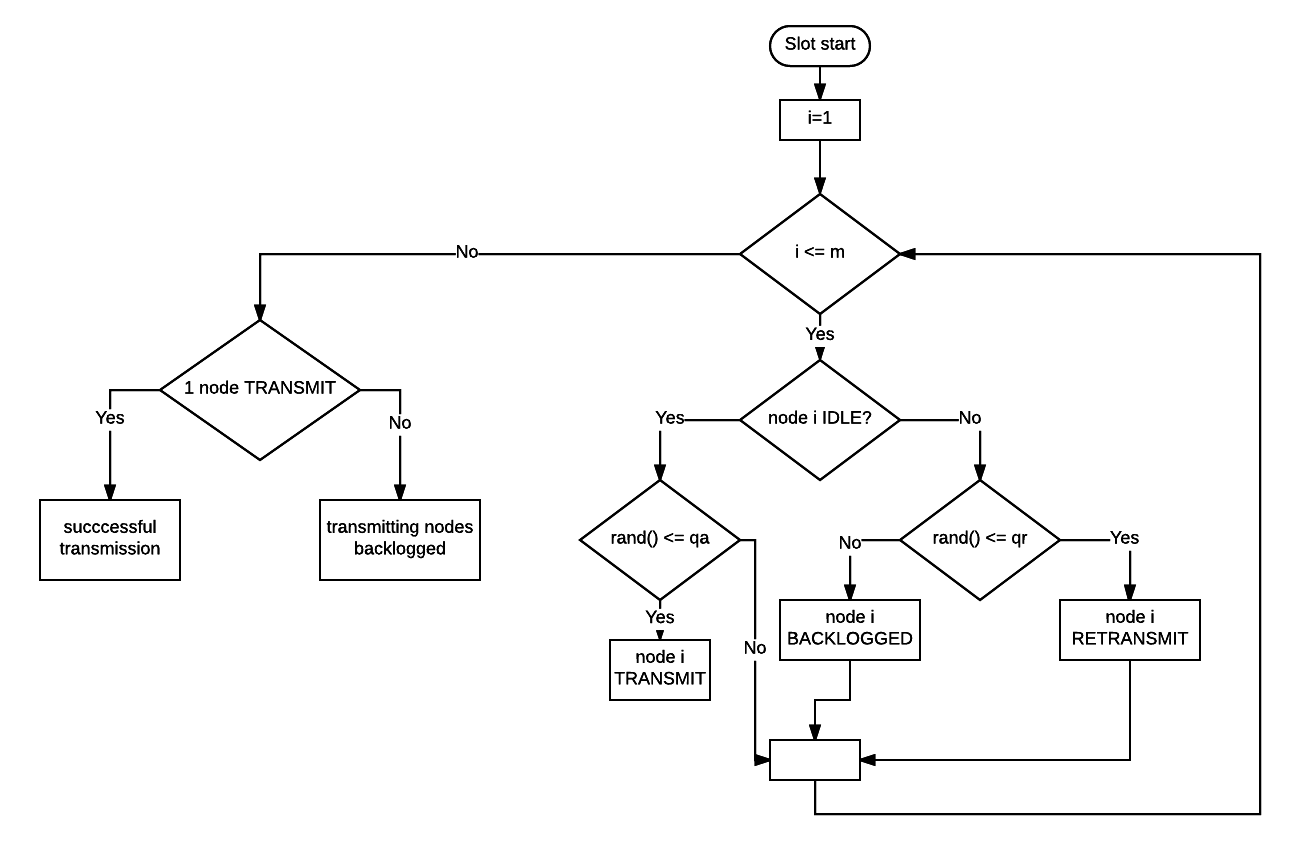
\includegraphics[width=.9\textwidth]{figures/flowchart.png}
\end{figure}

\subsection{$\lambda = 1/e, q_r = 0.01$}
\begin{figure}[h]
  \begin{subfigure}{.5\textwidth}
    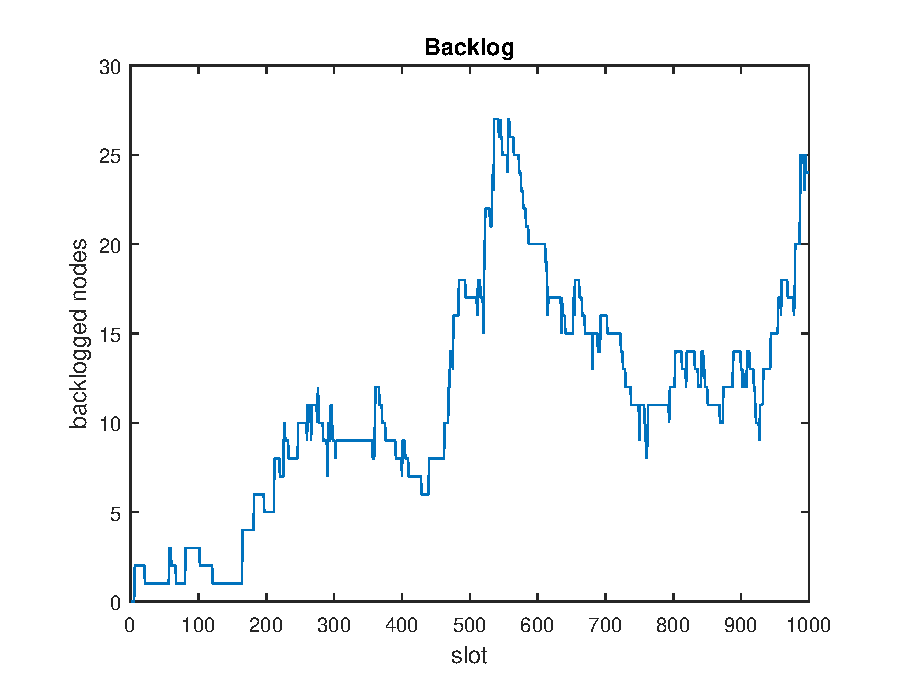
\includegraphics[width=\textwidth]{figures/backlog.eps}
    \caption{Backlog}
    \label{fig:backlog}
  \end{subfigure}%
  \begin{subfigure}{.5\textwidth}
    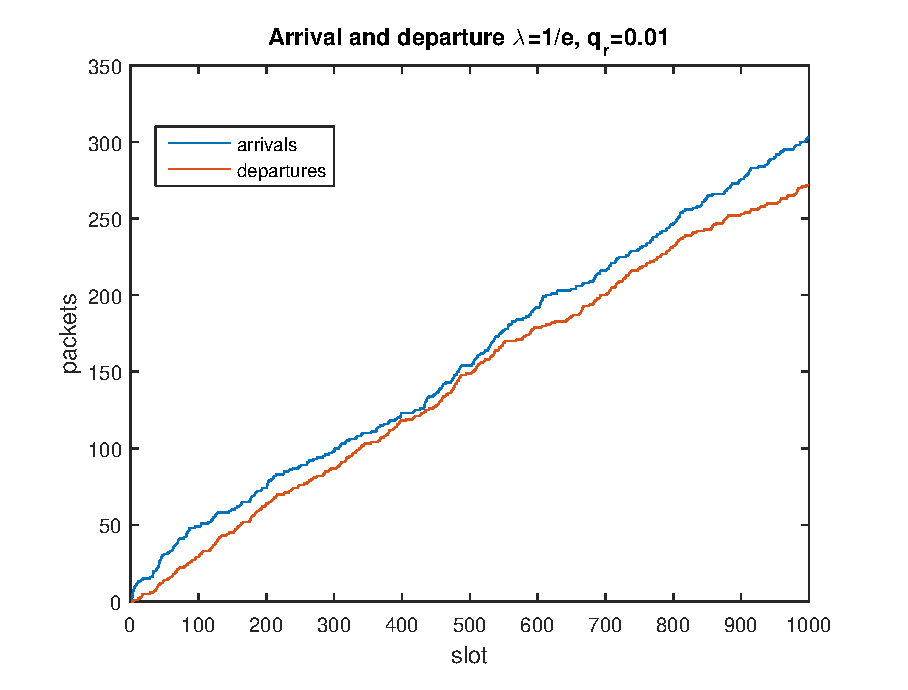
\includegraphics[width=\textwidth]{figures/arrival-departure-1.eps}
    \caption{Arrival and departure}
    \label{fig:arrival-departure}
  \end{subfigure}
  \caption{}
\end{figure}

3) In the first simulation the ALOHA protocol have been executed with retransmission rate $q_r=0.01$ and arrival rate $\lambda=1/e$. In figure~\ref{fig:backlog} the number of packets in the backlogged have been plotted. We can see that the backlog starts at zero and then increase. The backlog increases with one or more at a collision but it can only decrease by one step at a time since there can only be one succesful transmission at a time. This can be seen in the left graph. Figure~\ref{fig:arrival-departure} shows arrived packets (blue legend) and departured packets (red legend). The graph for arrived packets increase one step for each new arriving packet and the graph for departures increase one step at a time when a packet is successfully transmitted. The gap between these two graphs represents the delay of the system where a larger gap equals a longer delay. The horizontal distance between the two graphs at a $y=n$ is the delay for arriving packet number $n$. 

\begin{figure}[h]
  \begin{subfigure}{.5\textwidth}
    \centering
    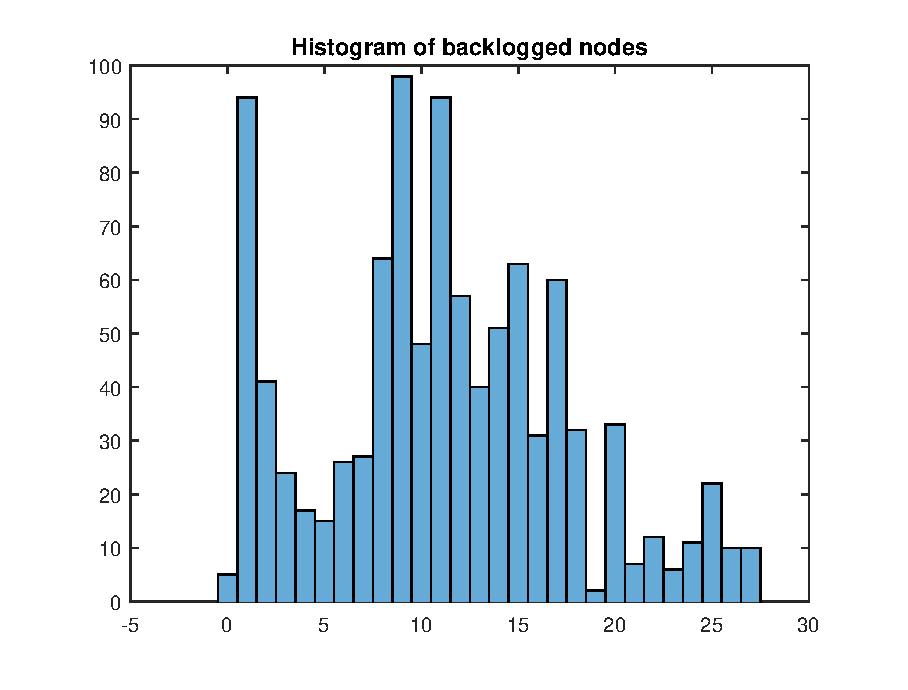
\includegraphics[width=\textwidth]{figures/hist-backlog.eps}
    \caption{Histogram of backlog}
    \label{fig:hist-backlog}
  \end{subfigure}%
  \begin{subfigure}{.5\textwidth}
    \centering
    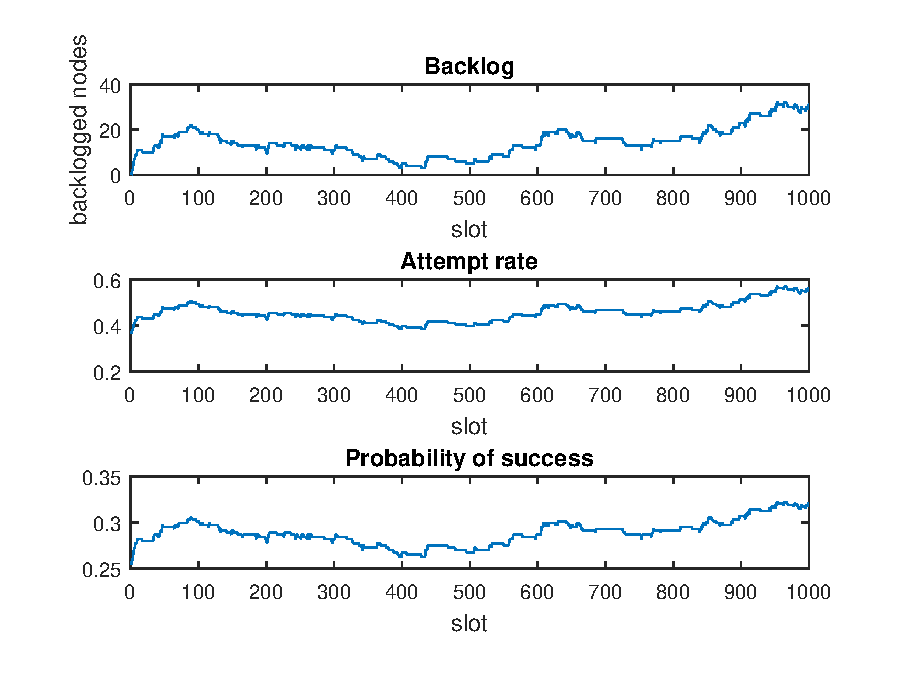
\includegraphics[width=\textwidth]{figures/backlog-attempt-probsuccess.eps}
    \caption{Backlog, attempt rate, and probability of success}
    \label{fig:backlog-attempt-probsuccess}
  \end{subfigure}
\end{figure}

4) By using the Matlab command \texttt{tabulate} we can obtain the steady-state probabilities of the Markov chain from the backlog. The expected number of backlogged nodes $N$ can then be calculated as $N = \sum_{n=0}^{m}{np_n}$, where $n$ is the number of backlogged nodes and $p_n$ is the probability of having $n$ backlogged nodes. From the simulation results the expected number of backlogged nodes was around 11. The attempt rate $G(n) = (m-n)q_a + nq_r$, and probability of success $P_s = G(n)e^{-G(n)}$ can be seen in figure~\ref{fig:backlog-attempt-probsuccess}. The rates depends on the backlog and have been calculated with the theoretical formulas for each slot. The average of the calculated probabilities of success is 0.28. Compared to the probability of success from the simulation which was 0.29, we may say that the estimation is good. 

\subsection{$\lambda = 1/2, q_r = 0.01$}
\begin{figure}[h]
  \begin{subfigure}{.5\textwidth}
    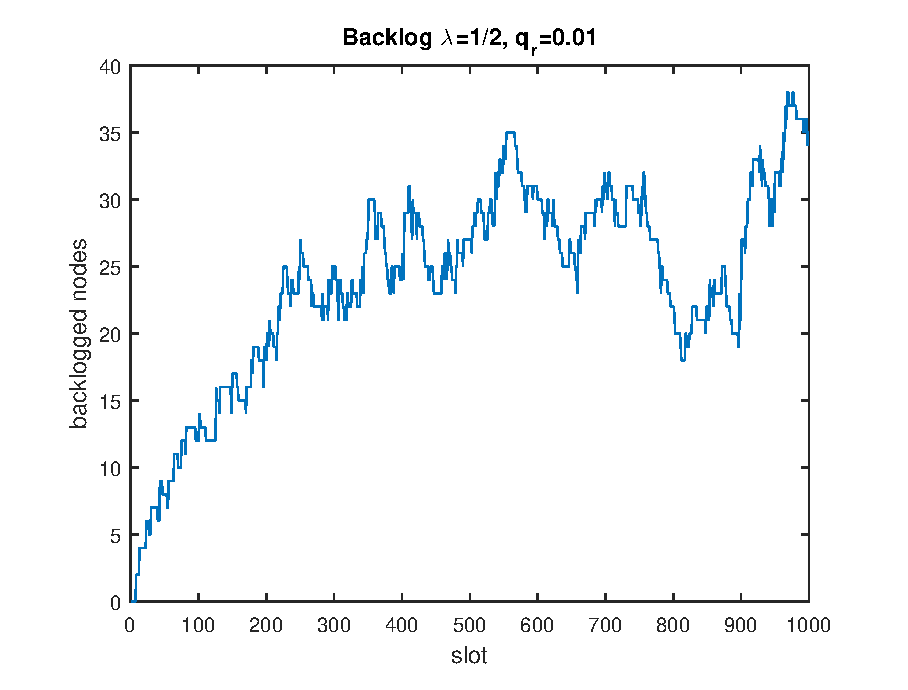
\includegraphics[width=\textwidth]{figures/backlog2.eps}
    \caption{Backlog}
    \label{fig:backlog2}
  \end{subfigure}%
  \begin{subfigure}{.5\textwidth}
    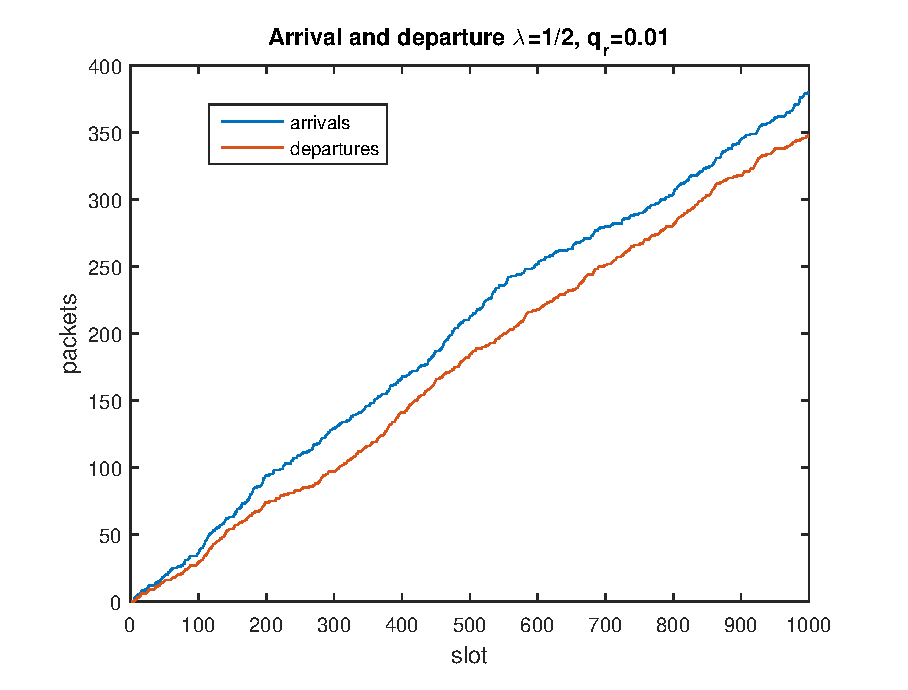
\includegraphics[width=\textwidth]{figures/arrival-departure-2.eps}
    \caption{Arrival and departure}
    \label{fig:arrival-departure-2}
  \end{subfigure}
  \caption{}
\end{figure}

In this run of the simulation $\lambda=1/2$ instead and $q_r$ is kept at $0.01$. this will increase the arrival rate and as we can see in figure~\ref{fig:backlog2} the backlog increases faster and the average number of backlogged nodes is also higher than in the previous plot. The delay have also increased since the gap between the graphs in figure~\ref{fig:arrival-departure-2} have increased. This is expected since now packets arrive at faster rate giving more collisions.\\\\\\\\

\subsection{$\lambda = 1/e, q_r = 0.1$}
In this run of the simulation $\lambda=1/e$, and $q_r=0.1$. This will make the backlog clear faster as we can see in figure~\ref{fig:backlog3-2}. Figure~\ref{fig:arrival-departure-3-2} shows that the delay is low and that packets depart very soon after arriving. However, sometimes we get unlucky where the backlog goes above a threshold and it will never clear and give no succesful transmissions as seen in figure~\ref{fig:backlog3}. This is also very clear in figure~\ref{fig:arrival-departure-3} where we can see that there is almost no successful transmission when the backlog becomes large.

\begin{figure}[h]
  \begin{subfigure}{.5\textwidth}
    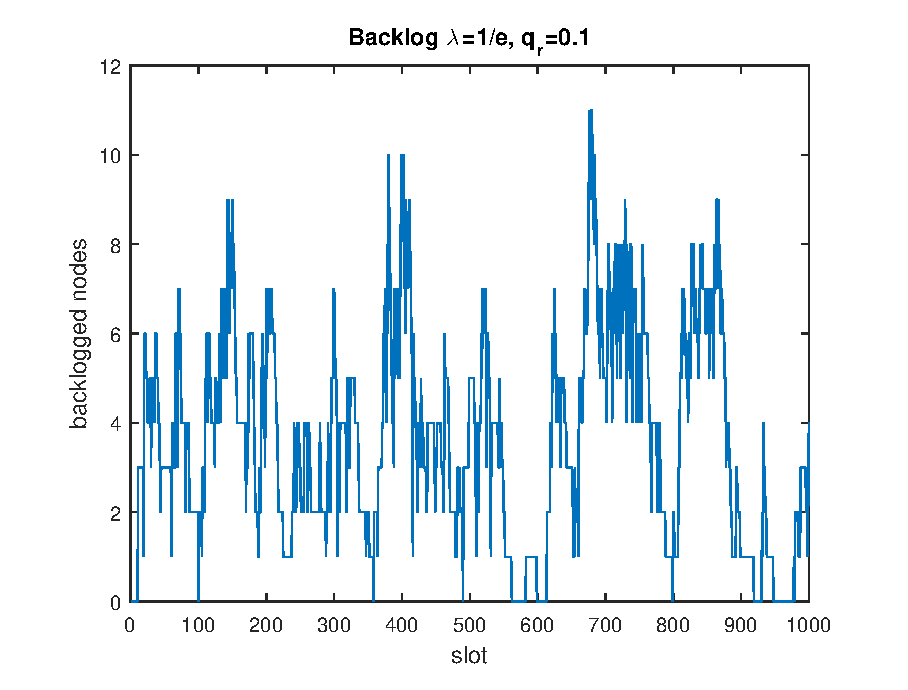
\includegraphics[width=\textwidth]{figures/backlog3-2.eps}
    \caption{Backlog}
    \label{fig:backlog3-2}
  \end{subfigure}%
  \begin{subfigure}{.5\textwidth}
    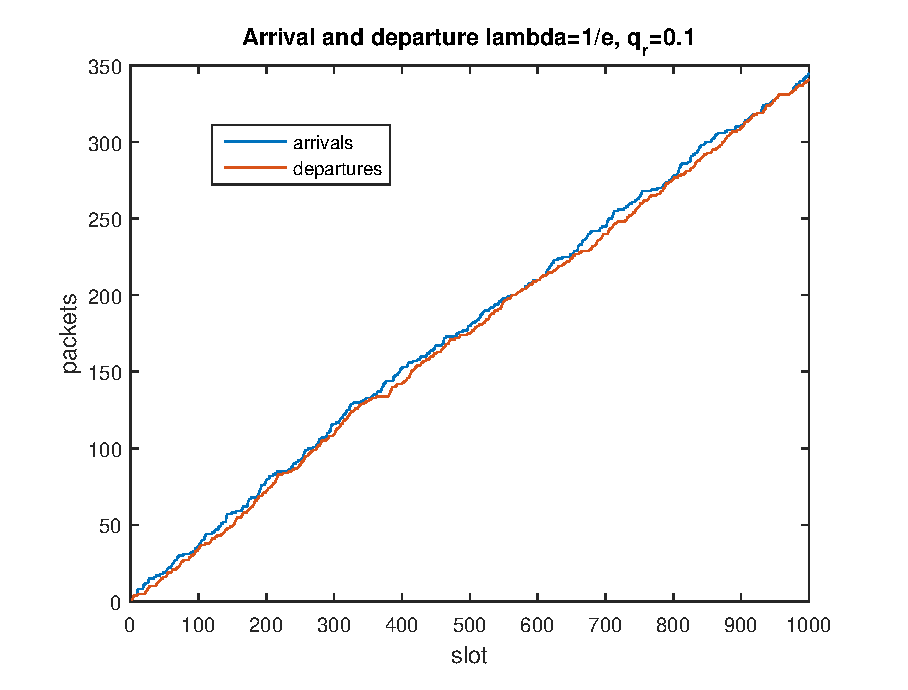
\includegraphics[width=\textwidth]{figures/arrival-departure-3-2.eps}
    \caption{Arrival and departure}
    \label{fig:arrival-departure-3-2}
  \end{subfigure}
  \caption{}
\end{figure}

\begin{figure}[h]
  \begin{subfigure}{.5\textwidth}
    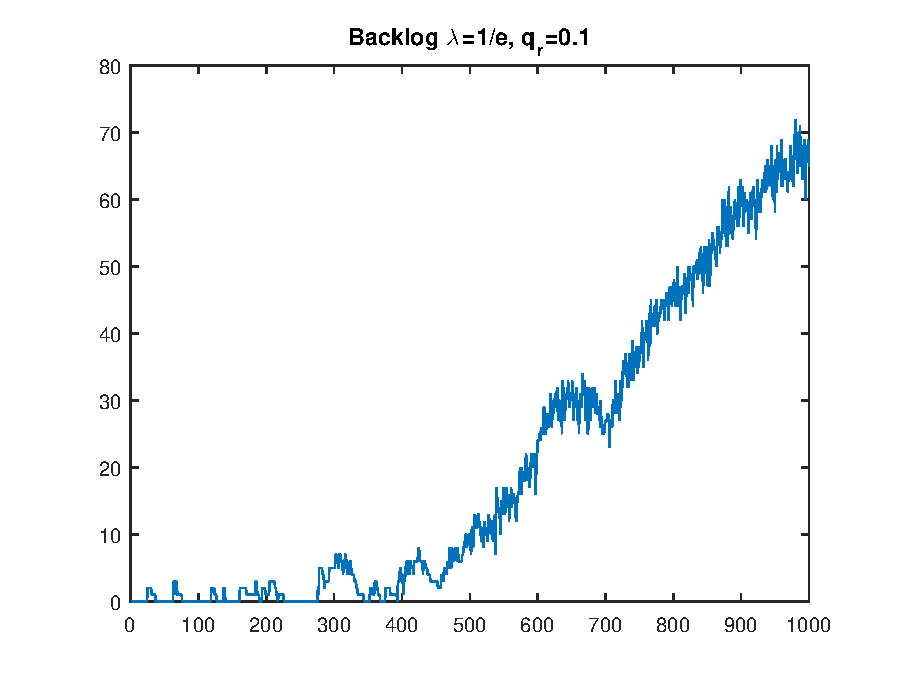
\includegraphics[width=\textwidth]{figures/backlog3.eps}
    \caption{Backlog}
    \label{fig:backlog3}
  \end{subfigure}%
  \begin{subfigure}{.5\textwidth}
    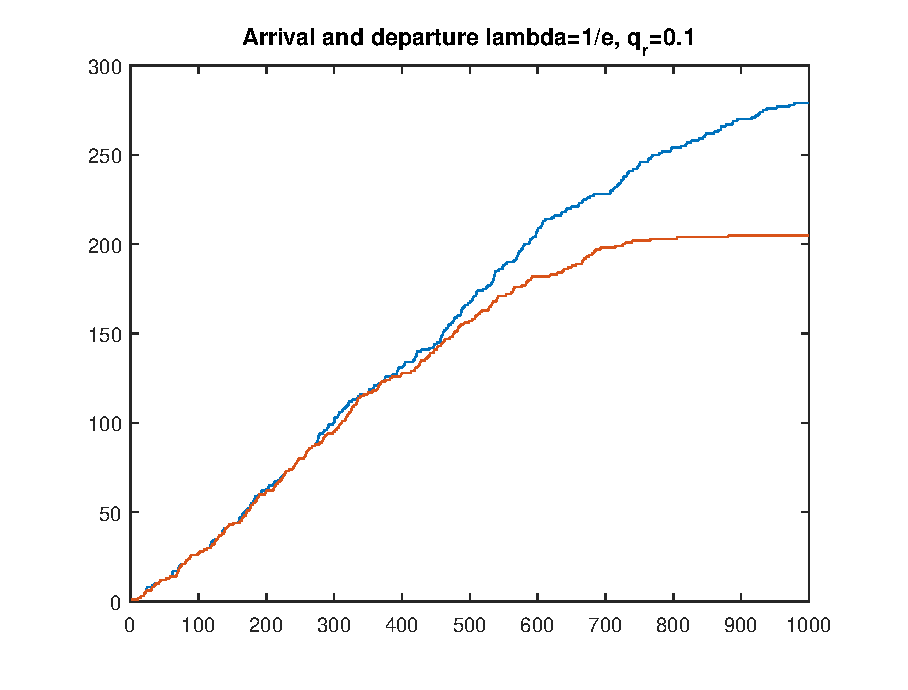
\includegraphics[width=\textwidth]{figures/arrival-departure-3.eps}
    \caption{Arrival and departure}
    \label{fig:arrival-departure-3}
  \end{subfigure}
  \caption{}
\end{figure}


\newpage

\section{Slotted ALOHA with Pseudo-Bayesian Stabilization}

In this section the simulations will be executed with the slotted ALOHA protocol, but now $q_r$ is adapted by the pseudo-bayesian stabilization. $\lambda=1/e$ is known.
\begin{figure}[h]
  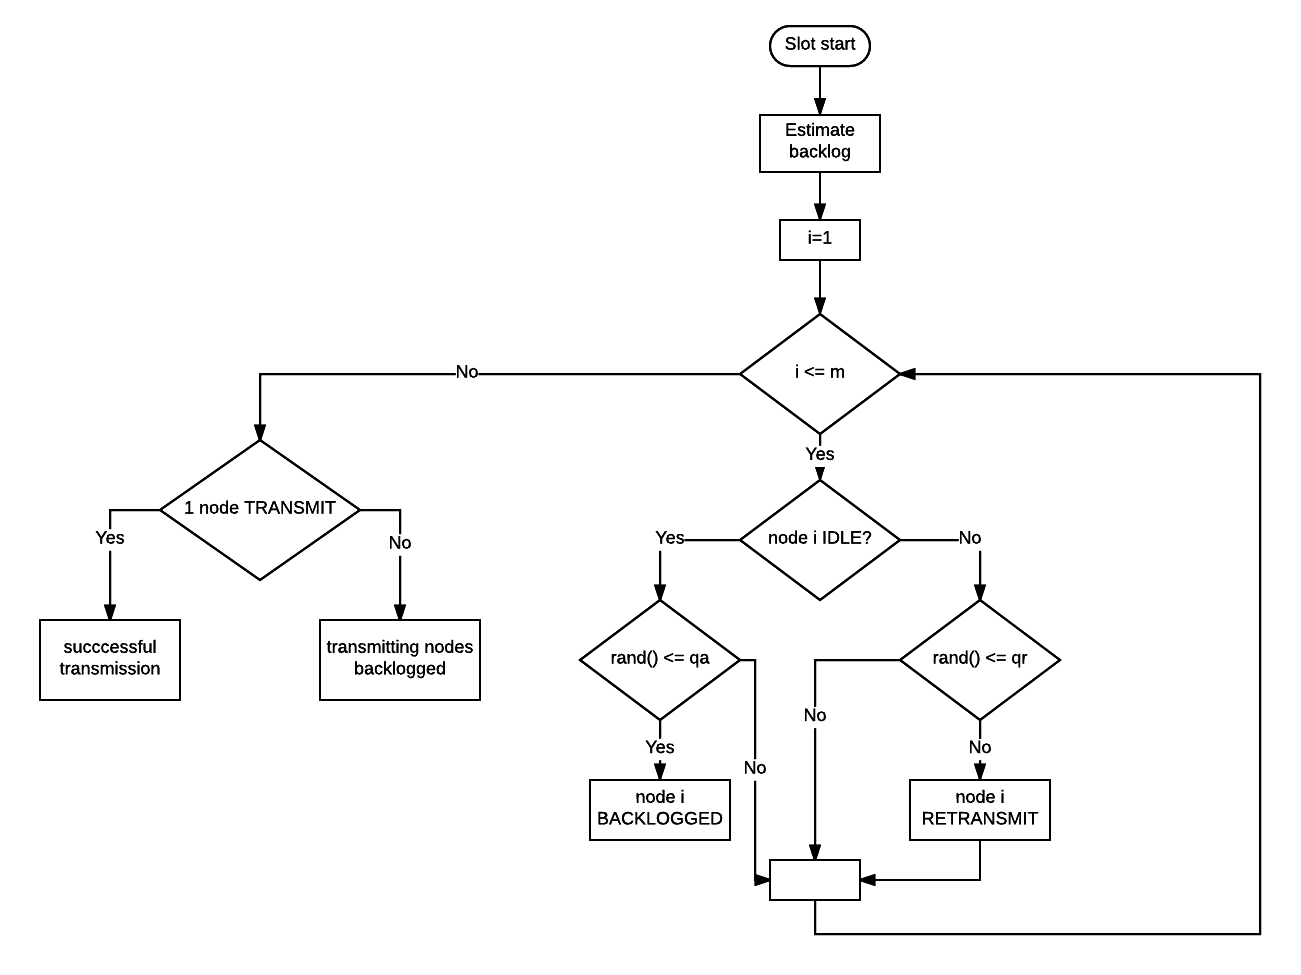
\includegraphics[width=.9\textwidth]{figures/flowchart-stabilized.png}
\end{figure}

\begin{figure}[h]
  \begin{subfigure}{.5\textwidth}
    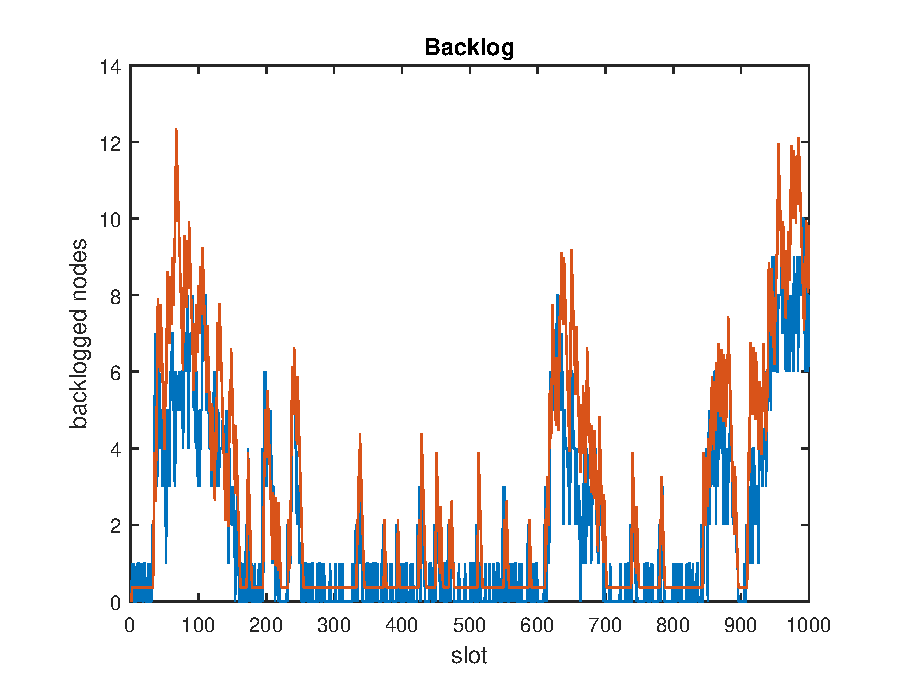
\includegraphics[width=\textwidth]{figures/backlog-stabilized.eps}
    \caption{Backlog}
    \label{fig:backlog-stabilized}
  \end{subfigure}%
  \begin{subfigure}{.5\textwidth}
    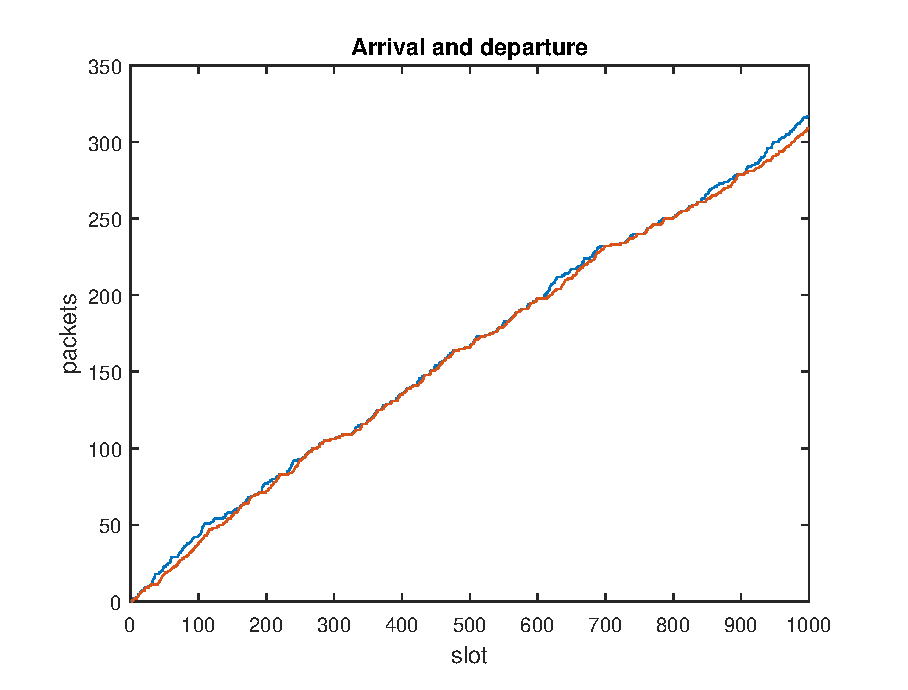
\includegraphics[width=\textwidth]{figures/arrival-departure-stabilized.eps}
    \caption{Arrival and departure}
    \label{fig:arrival-departure-stabilized}
  \end{subfigure}
  \caption{}
\end{figure}

With pseudo-bayesian stabilization the backlog will be estimated. Figure~\ref{fig:backlog-stabilized} shows the simulated backlog (blue) and the estimated backlog (red). As we can see the estimate follows the real backlog very good which will give a good retransmission rate. The delay is low as we can see in figure~\ref{fig:arrival-departure-stabilized} since the gap between the graphs is very small. This is an indication that the system is stable.

\begin{figure}[h]
  \centering
  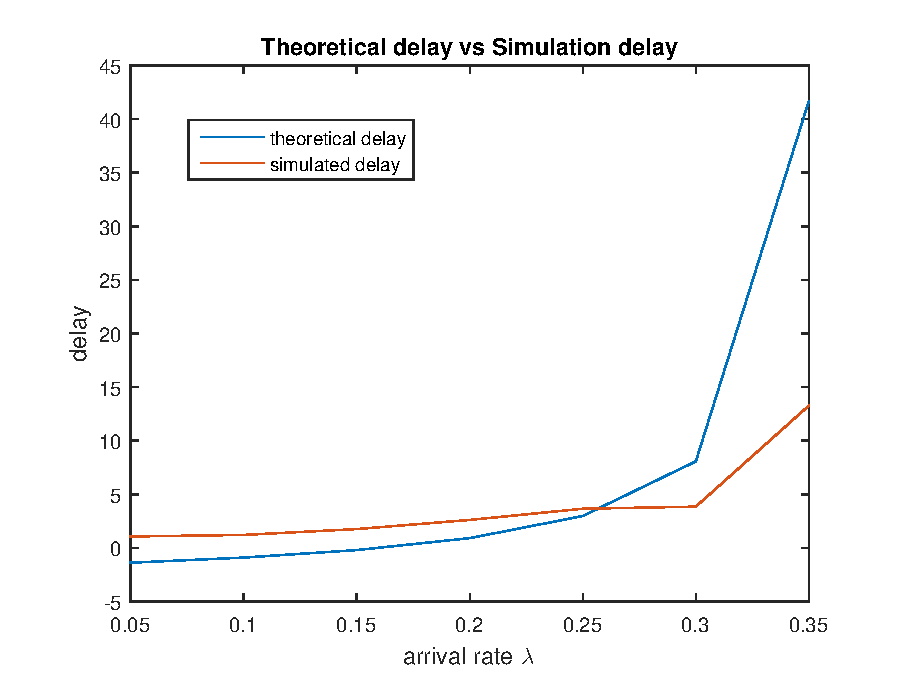
\includegraphics[width=.5\textwidth]{figures/approximate-delay.eps}
  \caption{Approximate delay}
  \label{fig:approximate-delay}
\end{figure}

The approximate delay of the system depends on the arrival rate $\lambda$. In figure~\ref{fig:approximate-delay} the approximated delay for successful packet transmission has been plotted. Both the delay from the formula (blue) and from the simulation results (red) can be seen for arrival rate $\lambda = 0.05:0.05:0.35$. The actual delay from the simulation result is almost the same as the theoretical delay for small arrival rates. But for larger arrival rates the actual simulation delay is smaller than the theoretical delay as we can see in figure~\ref{fig:approximate-delay}. 

\newpage
\appendix
\section{Slotted ALOHA}
\lstinputlisting{../slotted_aloha.m}

\newpage
\section{Slotted ALOHA with Pseudo-Bayesian Stabilization}
\lstinputlisting{../stabilized_slotted_aloha.m}

\newpage
\section{Plots}
\lstinputlisting{../plots.m}

\section{Utility functions}
\lstinputlisting{../attempt_rate.m}
\lstinputlisting{../average_delay.m}



\end{document}